\documentclass[a4paper,12pt,abstracton,titlepage]{scrartcl}
\usepackage{scrpage2}
\usepackage[utf8]{inputenc}
\usepackage[T1]{fontenc}
\usepackage[top=2.5cm, bottom=2.5cm, left=2.5cm, right=2.5cm]{geometry}
\usepackage[affil-it]{authblk}
\usepackage{lipsum}
\usepackage[hidelinks]{hyperref}
\usepackage{graphicx}
\usepackage[table,xcdraw]{xcolor}
\usepackage{longtable}

% code for generating glossary, from http://tex.stackexchange.com/a/5837/59718
\usepackage[acronym,toc]{glossaries}
\newcommand{\dict}[2]{%
  \newglossaryentry{#1}{name=#1,description={#2}}%
  \glslink{#1}{}%
}
\makeglossaries

% Here we set up the header, meta-information and front matter
\date{November 29, 2014}      %// Today's date will appear when this is commented out.
\newcommand{\version}{2.0}

% title page
\author{Maarten Baertsoen and Daniel S. C. Schiavini}
\affil{Open Universiteit Nederland, faculteit Informatica \\
	T61327 - Afstudeerproject bachelor informatica}
\title{Project Planning}
\subtitle{Useful feedback in the\\ Ampersand parser}
\publishers{Version \version}


% header
\pagestyle{scrheadings}
\setheadsepline{0.2pt}
\clearscrheadings
\automark[section]{chapter}
\ihead{M. Baertsoen and D.S.C. Schiavini}
\ohead{ABI Project Planning}
\cfoot{\pagemark}

% requirements
\newcommand{\req}[5]{~\\
	\begin{tabular}{|>{\columncolor[HTML]{C0C0C0}}p{2.5cm}|p{10cm}|}\hline
		\cellcolor[HTML]{9B9B9B}Requirement	& \cellcolor[HTML]{9B9B9B}\textbf{#2} \\\hline
		ID			& \texttt{#1} \\\hline
		Category	& #3 \\\hline
		Source 		& #4 \\\hline
		Description	& #5 \\\hline
	\end{tabular}~\\
}

%risks
\newcolumntype{R}{|>{\columncolor[HTML]{C0C0C0}}p{2,5cm}|p{2,2cm}|>{\columncolor[HTML]{C0C0C0}}p{2,2cm}|p{2,2cm}|>{\columncolor[HTML]{C0C0C0}}p{2,2cm}|p{2,2cm}|}
\newcommand{\risk}[1]{\cellcolor[HTML]{9B9B9B}Risk: & \multicolumn{5}{p{13,5cm}|}{\cellcolor[HTML]{9B9B9B}#1}}
\newcommand{\riskline}[1]{\multicolumn{5}{p{13,5cm}|}{#1}}
\newcommand{\riskhigh}{\cellcolor[HTML]{FE0000}High}
\newcommand{\riskmedium}{\cellcolor[HTML]{FFCB2F}Medium}
\newcommand{\risklow}{\cellcolor[HTML]{34FF34}Low}

% hyphenation
\hyphenation{
	gua-ran-tee
	pro-duct
	cor-res-pon-ding
	me-cha-nism
	know-ledge
	de-ve-lo-pers
	do-cu-men-ta-tion
	Schi-a-vi-ni
	Ba-ert-so-en}

% Now the document starts
\begin{document}
\maketitle
\newpage

\tableofcontents
\listoffigures
\listoftables
\clearpage

% !TEX root = ../Documentation.tex
\section{Introduction}
\subsection{Identification}
This document contains the domain \& techniques analysis of the project `Useful feedback in the Ampersand parser'.
The document is the milestone product of the project phase 3a for Daniel S.C. Schiavini, as specified in the project planning \citenac{plan}.

This document is part of the graduation project of the computer science bachelor at the Open Universiteit Nederland.
The project `Useful feedback in the Ampersand parser' is executed in collaboration with Maarten Baertsoen, with support of the supervisor Dr. Bastiaan Heeren and examiner Prof.dr. Marko C.J.D. van Eekelen.
The assignment is given by Prof.dr. Stef Joosten, who researches how to further automate the design of business processes and information systems by the development of the Ampersand project.

Ampersand is an approach for the use of business rules to define the business processes.
Users describe the business rules in a formal language (ADL), and Ampersand compiles those rules into functional specification, documentation and working software
prototypes.
The main objective of this project is to improve the feedback and maintainability of the Ampersand parser.
See \citenac{plan} for more details on the project.

\subsection{Goals}
\lipsum[3]

\subsection{Document overview}
\lipsum[4]
\clearpage
% !TEX root = ../Planning.tex
\section{Project description}
\label{sec:project-description}

\subsection{The Ampersand project}
In November 2003, the Business Rules Manifesto\cite{business-rules} was written, with the main purpose of declaring independence for business rules in the world of requirements.
The manifesto supports the vision of business rules as equivalent to requirements.
This is considered a radical change on how people see the world of business architecture.

In December 2010, Stef Joosten, Lex Wedemeijer and Gerard Michels published the paper `Rule Based Design', presenting the Ampersand approach.
The approach puts the rules in the center, using them to define the business processes.
Ampersand is named after the \& symbol with the desire of realizing results for both business and IT, in an efficient and effective way.

In 2011, the Ampersand compiler was created as an open source project.
Since then, the compiler has been improved and applied in both business and academic contexts.
The Ampersand end-users write business rules in a specific language (ADL), and compile that specification into functional specification, documentation and working software prototypes.
\dict{ADL}{Ampersand Design Language}%
These rules are based on agreements between the different stakeholders.

The theory behind Ampersand has been throughly studied, and is based on mathe\-matical concepts, e.g. Relational algebra and Tarski's axioms.
Using this compiler, users write the requirements in ADL and generate all the system specification independent of the platform.
The main advantage is that the requirements consistency and traceability are always correct (and even provable), from the lowest level up to the front-end.
The requirements are presented to stakeholders in natural language, guaranteeing that any business expert who knows the context can validate the requirements.
\autoref{fig:generation} depicts the artifacts generated by the Ampersand compiler.
%
\begin{figure}[htb]
	\centering
	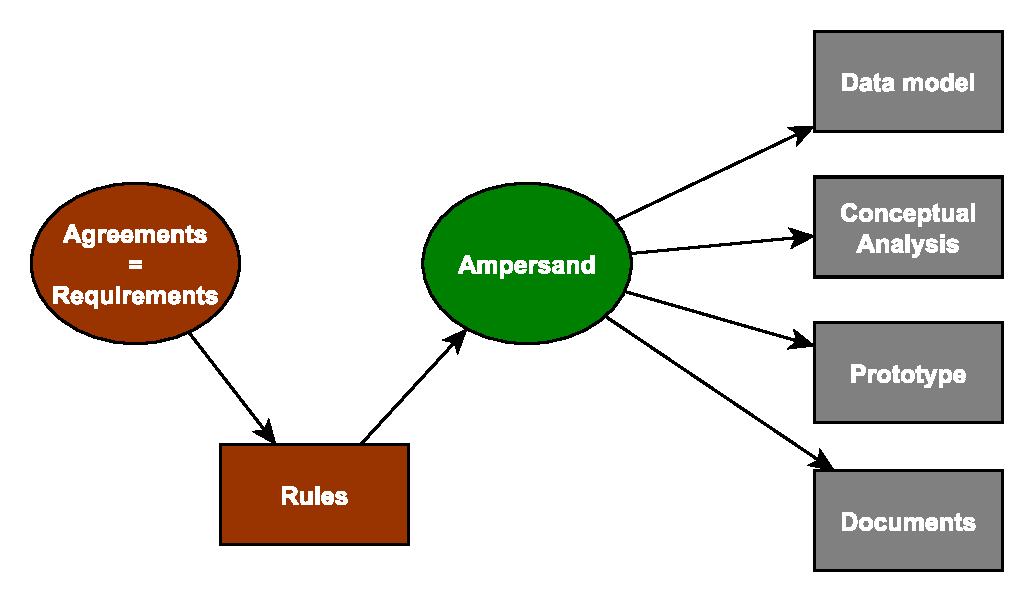
\includegraphics[width=0.7\textwidth]{Figures/Generation}
	\caption[Generated artifacts]{The Ampersand approach generates different artifacts based on the business rules}
	\label{fig:generation}
\end{figure}

\subsection{Project architecture and components}
\label{subsec:architecture}
The compiler developed for the Ampersand research project runs in several steps.
Thence the Ampersand compiler is also divided in several subcomponents:
\dict{P-structure}{The parse-tree generated by the Ampersand parser, used as input for the type checker.}%
\dict{A-structure}{The ADL code generated by the Ampersand type checker, used as input for the calculator component.}%
\dict{ADL-structure}{See A-structure.}%
\dict{F-structure}{The functional structure generated by the Ampersand calculator, used as input for the different output modules.}%
\begin{description}
	\item[Parser:] This component receives the ADL code as input, and parses that code into a parse-tree (also known as P-structure).
	\item[Type checker:] The Ampersand type checker receives the P-structure as input and converts it into a relational algebra format, suitable for manipulation (also known as A-structure or ADL-structure).
		 The semantics of ampersand are expressed in terms of the A-structure.
	\item[Calc:] The Calc component receives the A-structure as input, and manipulates it according to the research rules, generating the functional structure (also known as F-structure).
		The F-structure contains all design artifacts needed to write a specification and generate the output.
	\item[Output components:] All design artifacts present in the F-structure are ready to be rendered.
		Several components use this data structure to generate the wished output.
		The output components currently implemented (and their output formats) are the following: 
		\begin{itemize}
			\item Atlas (HTML interface);
			\item Revert (Haskell source);
			\item Query (prototype generation);
			\item Documentation Generator (Pandoc structure).
		\end{itemize}
\end{description}
%
The complete architecture is depicted in \autoref{fig:architecture}.
The part of this architecture relevant for this project is depicted in \autoref{fig:data-flow}.
%
\begin{figure}[htb]
	\centering
	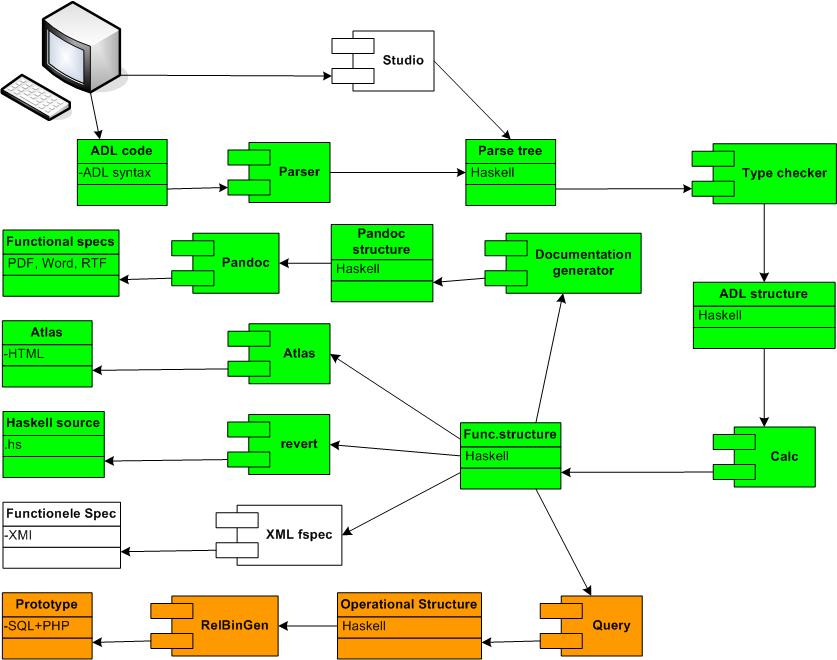
\includegraphics[width=\textwidth]{Figures/ADL_systeemarchitectuur}
	\caption[Architecture of the project]{Architecture of the project, showing where the parser fits in the Ampersand system}
	\label{fig:architecture}
	\small
	The components in green background are part of the Ampersand compiler.
	Components in orange are part of the Ampersand Prototype compiler.
	Finally, components in white background are future components, not yet implemented.
\end{figure}
%
\begin{figure}[htb]
	\centering
	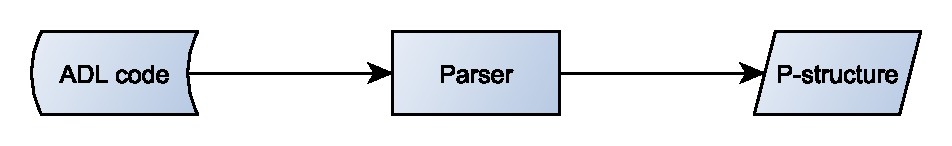
\includegraphics[width=0.5\textwidth]{Figures/Architecture}
	\caption{Relevant data flow for the Ampersand parsing component}
	\label{fig:data-flow}
\end{figure}

\subsection{Current situation}
The end-to-end process of the ampersand project, from compiling towards the generated artifacts is correct, however there is a major improvement topic identified in the first step, the parsing of the input scripts.

One of the main complaints from users is the quality of the errors generated by the Ampersand parser making it though for the end users to correct faulty ADL statements.
Since the beginning of the project, the parser subcomponent never received special attention, and it has not been analyzed for improvements.

In order to generate better, useful and to the point error messages, it is assumed that a complete refactoring of the parser will be necessary.
The main challenge is to choose the correct kind of architecture and libraries in order to generate the most user-friendly messages possible.

Besides the main project task of improving the parser's feedback, a list of user wishes has accumulated over the years.
The main customer and other users would appreciate if as many wishes as possible could be fulfilled.

\subsection{Goals of the project}
\label{subsec:project-goals}
The main objective for the graduation project is to implement useful feedback in the Ampersand parser.
In order to achieve this goal, the following research \& analysis activities will take place:
\begin{itemize}
	\item Analysis of user-friendly messages in compilers;
	\item Comparison of different Haskell parsing libraries (also for pretty-printing);
\end{itemize}
%
Additionally, the following activities may also take place:
\begin{itemize}
	\item Researching tools and techniques in Haskell for improving the software quality (e.g. testing and error messages);
	\item Analysis of the current development environment in relation with software engineering principles such as continuous delivery/integration;
	\item Recommending improvements for the overall software quality;
\end{itemize}
%
In case the new parser is successfully implemented and accepted, while the project members still have time budget available, the list of open user wishes issues can be addressed.
Some of these wishes are substantial, so that most of them cannot be fulfilled during the graduation project.
The current list of open issues has been provided\cite{open-issues}, although it must be clear that the issues are strictly seen as lower priority.
See also \autoref{sec:requirements} for the list of high-level requirements.

\subsection{Project environment}
The Ampersand project is used in the following environments, for different users:
\begin{description}
	\item[Research:] The Ampersand project is part of a research domain on the use of business rules for software design;
	\item[Academic:] Ampersand is used as main tool in the course `Ontwerpen met bedrijfsregels' (code T18321) from the Open Universiteit Nederland;
	\item[Business:] The compiler is used in business environments to design and develop real world business software.
\end{description}

\subsection{Critical success factors}
\label{subsec:success-factors}
The following factors are critical for the project's successful completion.
Each critical success factor is covered by one or more measures outlined in this project plan:
\begin{description}
	\item[Maintainability:] the code shall at least be as maintainable as the current Ampersand code.
		It is known however that maintainability is hard to measure (see also \autoref{sec:risk-management}).
	\item[Production code:] the implemented functionalities shall be integrated into the master branch for production use;
	\item[Users context:] in order to provide useful feedback, the user context wherein the Ampersand compiler is used needs to be well understood, and the improvements must have extra user value. 
		Just like maintainability, useful feedback is a hard to measure topic, this risk is listed in \autoref{sec:risk-management} and will be addressed in phase 3c (research context).
	\item[Communication:] Independent on how good the project results are, if the solution is put into production without proper communication and documentation leading to confused and demotivated users, the project will be perceived as a failure. 
	Although the project aims to add the feedback in the ampersand parser as transparent as possible, the final customer and user perception remains a critical success factor of this project;
\end{description}
%
The syntax of the Ampersand grammar is written in the the EBNF notation.
Any changes to the syntax must be documented according with this notation.
The notation can also be added as comment in the source code, in order to make clear that all the grammar is implemented completely and correctly.

\subsection{Objectives and commitments}
Besides the project goals described in \autoref{subsec:project-goals} and the customer goals described in \autoref{subsec:success-factors}, the project members declare herewith to have the following objectives and commitments fulfilled by the end of this graduation project:
\begin{description}
	\item[Customer:] The primary objective is to deliver a well-working and maintainable piece of software that will help the customer.
	\item[Users:] Another important goal is to make the software more user friendly, and so improve the usability.
	\item[Knowledge:] Building up knowledge is the main reason why one starts a bachelor study.
		As such it is important do learn more about functional programming, Haskell, compilers, business rules and research in general.
	\item[University:] Hopefully the final thesis will be of use for the university and other students.
	\item[Graduation:] As this is a graduation project, it is natural to have the graduation as an important objective.
\end{description}

\clearpage
% !TEX root = ../Planning.tex
\section{Project approach (M)}
\label{sec:project-approach}
Just like any other project, this project needs a fit-for-use approach. 
This section 'project approach' summarizes the project methodology we will apply together with an exhaustive overview of the project planning, milestones and corresponding deliverables.
\subsection{Project methodology}
The main drivers to determine our project methodology is based on the kind of deliverables that needs to be produced due to this project, more specific, the actual technical realization of the project.

We can group the technical realization into 2 categories:
\begin{enumerate}
	\item The introduction of a new error message approach to provide clear and useful error messages and warnings towards the end-users
	\item Stand alone modification points toward the Ampersand Parser based on
	\begin{enumerate}
		\item Reported issues
		\item Enhancements
		\item Extensions
	\end {enumerate}
\end {enumerate}

Given the stand alone aspect of the modification points, the use of a scrum based approach is quite obvious as we already have a product backlog of topics which can be taken up independently of each other. 


The error messages need somewhat more attention to guarantee that we build up a solid error message architecture. 
The project team will therefore realize a Proof-of-Concept to demonstrate the correct approach and base architecture. 
After validation of this POC, the project team will realize the error message architecture and actual implementation in a scrum like approach.
More information on the scrum like approach is described in section ‘Project realization’.



Within this project methodology, following aspects are identified as important to guarantee a qualitative project within time, budget en corresponding to the agreed on project scope : 
\begin{enumerate}
	\item Project management
	\item Knowledge acquisition 
	\item Project realization approach
	\item Integration \& release
	\item Testing \& validation
	\item Communication
	\item Documentation
\end {enumerate}

All these approach topics are fully documented within this project plan.


\subsection{Project phases}
 \begin{enumerate}
	\item Phase 2 - Task allocation and Project plan
	todo: description of phase
	\item Phase 3a - Domains \& Techniques
	todo: description of phase
 	\item Phase 3b - Investigation context (todo: find good translation for 'Onderzoekscontext)
	todo: description of phase
 	\item Phase 3c - Design \& implementation
	todo: description of phase
 	\item Phase 3d - Project documentation
	todo: description of phase
	\item Phase 4 - Project closure and final project presentation	todo: description of phase
\end {enumerate}

\subsection{Project planning, milestones and corresponding deliverables }
The project is planned based on the project milestones and the detailed project planning. The milestone will be formalized by the delivery of their corresponding deliverables

A commitment is given by the project team to adhere to the following milestone planning, officiated by the delivery their corresponding deliverables, grouped by their corresponding project phase:

 \begin{enumerate}
	\item Phase 2 - Task allocation and Project plan
 	\begin{enumerate}
		\item Delivery of the detailed project plan 			- 	13/11/2014
		\item Detailed allocation of tasks within the project team 	- 	13/11/2014
	\end {enumerate}
	\item Phase 3a - Domains \& Techniques
 	\begin{enumerate}
		\item Delivery of scientific article by Daniel			- 	03/12/2014
		\item Delivery of scientific article by Maarten  			- 	03/12/2014
	\end {enumerate}
 	\item Phase 3b - Investigation context (todo: find good translation for 'Onderzoekscontext)
 	\begin{enumerate}
		\item Detailed report of the 'investigation context)  		- 	29/04/2014
	\end {enumerate}
 	\item Phase 3c - Design \& implementation
 	\begin{enumerate}
		\item Analysis \& design documents  				- 	30/03/2014
		\item Test report  							- 	20/03/2014
		\item Source code  							- 	27/03/2014
		\item The actual release of the realized product  		- 	20/04/2014
		\item IT documentation  						- 	20/03/2014
		\item User documentation \& user manual  			- 	20/03/2014
	\end {enumerate}
 	\item Phase 3d - Project documentation
 	\begin{enumerate}
		\item Project documentation document				- 	04/05/2014
	\end {enumerate}
	\item Phase 4 - Project closure and final project presentation
 	\begin{enumerate}
		\item Project essay							- 	20/05/2014
		\item Project presentation						- 	date to be jointly determined, final due date 29/05/2014
	\end {enumerate}
\end {enumerate}

The project activities will be managed in a detailed project planning by the project team, and the status will be shared during project alignment meetings.
Deviations, changes and issues within the project plan will be managed by the project team itself, in full openness towards the project stakeholders. 
As long as the changes to the detailed project plan aren't  compromising the milestone plan, the project is considered to be 'in control'. 

Any deviation of the project plan (due to risks, delays, issues,...) that can have an impact on the project milestone planning will be reported even before they really hit the project plan. 
This way, all project stakeholders will be informed and can cooperate in the corrective actions.





\clearpage
% !TEX root = ../Planning.tex
\section{Project management}
\label{sec:project-management}
This sections describes the project management approach and used techniques to guarantee project success.
As the project team consists only out of 2 team members, special attention is given to make the project management approach holistic but light.
Holistic to assure that all important aspects with regards to the management of this project are properly covered and lightweight to avoid that the project team loses time in handling unnecessary tasks which only have added value in larger project teams.

\subsection{Project governance / roles \& responsibilities}
We distinguish 5 different project parties in the project environment:
\begin{description}
	\item[The project team]
	The project team consists out of Daniel Schiavini and Maarten Baertsoen.
	This team takes the full responsibility for the day to day project management as well as the actual delivery of all project work products consisting out of
	\begin{enumerate}
		\item The actual Haskell program code in full conformity with the coding conventions
		\item Exhaustive code documentation
		\item All necessary, final and intermediate, deliverables to ensure project's success such as: project planning, action/issues/risks lists and intermediate status reports based on the project methodology.
	\end {enumerate}
	The full list of all work products with their corresponding description is included in \autoref{sec:project-approach}.
	
	\item[The project supervisor]
	The project supervisor is Bastiaan Heerlen.
	He is the main contact person for the project team.
	It is the role of the project supervisor to monitor the project team on a regular basis as well as to provide support and guidance to the project team members both on content and approach.
	It is the responsibility of the project team to send project status updates towards the project supervisor; these status updates will form the basis for the regular alignment meetings.

	During project execution, it might occur that the effort needed to meet the customer expectations is way over the foreseen budget, measured in hours, of the project.
	Should this situation occur, the supervisor will facilitate customer alignments to adjust the customer's expectations.

	All efforts spent are reported on a regular basis to the supervisor who will track the spent effort to make sure that every aspect of the project receives the proper attention it deserves.

	\item[The customer]
	The project will deliver an actual product with all corresponding documentation in a clear and controlled way.
	The customer's satisfaction is one of the key success factors of this project.

	Although this project is conducted in an educational environment, the customer shall be treated just like he would be in a professional environment.

	\item[End-Users]
	The Ampersand Parser is actively used by several users groups.
	Although these user groups are not addressed directly, they will be affected when the project team releases new topics in the Ampersand Parser.
	All necessary communication and change management techniques applied to support the introduction of new functionality are described within this document.

	All topics in which the end user groups are involved need to be carefully aligned with the customer as it is the customers responsibility to keep the Ampersand Parser up and running and in good shape.
	Introduction of bugs, unclear functionality or even the total unavailability will harm the customer reputation.

	\item[The examiner]
	Last but not least, the examiner will evaluate all aspects of the project to which he will grant a score.
	These sub-score will be used to determine the final and individual course result.
	It's obvious that the customer's satisfaction is one of the main benchmarks, however the examiner will also evaluate the used project approach, academic skills and personal investigation areas.
\end {description}

\subsection{Communication}
\label{subsec:communication}
Regular alignment and communication sessions are foreseen within the project.
The communication plan described below identifies the way the project team will align and communicate with the involved project parties.

\subsubsection{Internal}
The project team members, Daniel Schiavini and Maarten Baertsoen will align on a weekly basis.
During this meeting, following topics will be discussed:
\begin{enumerate}
	\item Tasks done
	\item Tasks due
	\item Alignment on and assignment of the upcoming project tasks
	\item Actions
	\item Issues \& Risks
\end {enumerate}
%
Given the project size of the team, Daniel and Maarten will communicate informally on a regular basis besides this recurrent weekly meeting.

\subsubsection{OU}
\dict{OU}{Open Universiteit Nederland}%
A recurrent meeting between the project supervisor and the project team is planned every 3 weeks.
This meeting is an official feedback meeting, from team to supervisor, providing the full status of the project encompassing all important project aspects such as progress, issues and risks.

During these meetings the supervisor will monitor and steer the project progress and will check the proper project management by consulting the project's statistics.

All documents will be delivered to the project supervisor at least 24 hours before the actual meeting to allow the project supervisor to perform an in depth review.

\subsubsection{Customer}
The sessions with he customer will be planned carefully, both on timing and content, to make sure that the customer is not disturbed too much with project questions not relevant for them as a customer, but without losing the insight in the customer's needs.

The main principle to distinguish between the questions that can be posed to the customer or not, is by reflecting this project to a professional business project.
Every question or issue that should be handled by a professional project team, based on knowledge and experience, will be handled internally within this project as well.

All questions, issues and status updates towards the customer will be listed by the project team and will be revised with the project supervisor to assure to customer meetings are efficient, clear and most importantly, that these meetings provide the customer a trustful feeling regarding the project.

\subsection{Time keeping}
The project team members will record every effort they have spent on the project an overview over:
\begin{enumerate}
	\item Date
	\item Phase
	\item Domain
	\item Member
\end {enumerate}
This overview will be shared with the project supervisor on a regular basis and whenever requested.

\subsection{Project reporting}
The project team will share periodic status updates during the project, this reporting will cover following project aspects:
\begin{enumerate}
	\item General project status
	\item Timing
	\item Results achieved
	\item Budget (spent hours)
	\item Risks and issues
	\item Quality
	\item Focus for the upcoming weeks
\end {enumerate}

\subsection{Quality assurance}
The customer's perception of the project quality will have a tremendous impact on the overall rating of the project deliverables and therefore, it is for the project team of utmost importance to demonstrate the measures taken to guarantee project success.

Having correct quality assurance processes is not sufficient when these are not used on a day-to-day basis.
The project team will present quality reports towards the project supervisor and the customer to gain their confidence that the project team will deliver the promised quality.

Following topics will be monitored and reported: 
\begin{enumerate}
	\item Issue handling
	\item Follow up of actions
	\item Release procedures to put project coding into the production environment
	\item Communication \& change management
	\item Test management
	\item Tool effectiveness
	\item Documentation management
\end {enumerate}

\subsubsection{Process quality \& monitoring}
The used project management processes must be both light and effective.
The project team will monitor the effectiveness of these processes on a regular basis and carry through useful changes after alignment with the project supervisor.

\subsubsection{Deliverables quality \& monitoring}
Each project deliverable will be reviewed by the project team member's counterpart within the project team.

Where needed, several revision iterations will be foreseen until the project team comes to an agreement regarding the sufficient quality level of the deliverable.
Deliverables approved within the project team will be shared with the project supervisor who can perform an additional quality check before the deliverables are shared with the customer and the project examiner.

Each delivery towards the customer can be followed by a subsequent revision phase to perform a final fine-tuning to assure customer satisfaction.

Especially for the work items that consist out of programmed code, a thorough review will be done to assure that the programmed code is in line with the coding conventions as delivered by the customer (see \autoref{subsec:coding-conventions}).

\clearpage
% !TEX root = ../Planning.tex
\section{High-level requirements (D)}
\label{sec:requirements}
In this section, a list of known requirements is given.
Please note that because the project plan is made in the beginning of the project, only the highest-level requirements can be described.
Also note that the project will be executed in an iterative/agile way, so the requirements will change, and when they do this document might be not updated.

~\newline\noindent
In this section, the abbreviation NAP is used, with the meaning ``new Ampersand Parser''.
\dict{NAP}{Ampersand Parser}%

\subsection{Functional requirements}
\req{PL-FUN-010}{Ampersand code base}{
	The NAP shall be implemented in the Ampersand code base.\\
	Note: This also means that NAP shall be implemented in the Haskell programming language, and will use the same compiler as Ampersand does.}

\req{PL-FUN-020}{User-friendly errors}{
	The NAP shall give user-friendly error messages for the most common parsing errors.\\
	Note: Discovering which errors are the most common is part of the assignment.}

\req{PL-FUN-030}{Command-line interface}{
	The NAP shall only have a command-line interface.}

\req{PL-FUN-040}{Windows environment}{
	The NAP shall run in the Microsoft Windows 7 operational system.}

\req{PL-FUN-050}{Git repository}{
	The NAP code shall be managed in the ``AmpersandTarski/ampersand'' GitHub repository, in the ``ABI\_Parser'' branch.}

\req{PL-FUN-050}{P-structure}{
	The NAP code shall generate the P-structure in the same way the old Ampersand parser currently does.}

\subsection{Non-functional requirements}

In case the new parser is successfully implemented and accepted, while the project members still have time budget available, the list of open user wishes issues can be addressed.
Some of these wishes are substantial, so that most of them cannot be fulfilled during the graduation project.
The current list of open issues has been provided\cite{open-issues}, although it must be clear that the issues are strictly seen as lower priority.

\clearpage
\section{Knowledge acquisition (-)}
\label{sec:knowledge-acquisition}

\subsection{Research context}
Some ideas by Bastiaan:
\begin{itemize}
  \item more info on ampersand users
  \item user-friendly error messages (specific to compilers or not)
  \item parser-libraries
  \item Stef's research (3a)
  \item Haskell parsers (e.g. Helium), monadit or combinators
\end{itemize}

\subsection{Domain \& technology}
\subsubsection{Part Daniel}
\lipsum[1]

\subsubsection{Part Maarten}
\lipsum[1]

\subsection{Knowledge documentation}
\lipsum[1]

\clearpage
% !TEX root = ../Planning.tex
\section{Project realization (-)}
\label{sec:project-realization}
\subsection{Coding conventions}
\lipsum[1]
\subsection{Scrum approach}
\lipsum[1]
\subsection{Validation}
\lipsum[1]
\clearpage
% !TEX root = ../Planning.tex

\section{Integration \& release}
\label{sec:integration-release}
\dict{branching}{Branching is the duplication of an object under revision control so that modifications can happen in parallel along both branches.}%
\dict{merging}{The reintegration of a branch into the original code}%
The code changes of this project will be done in a separate branch (\texttt{ABI\_Parser}) of the Ampersand GitHub repository (\texttt{AmpersandTarski/ampersand}).
In the end of each sprint, the project members will evaluate whether the integration into the master branch is advised.
If so, the following steps will be taken:
\begin{enumerate}
	\item The code has already been merged and tested in the project branch.
	\item The project manager shall send a notification via e-mail to the customer, including the test documentation and any other applicable information, such as the commit identifier (see \autoref{subsec:test-documentation}).
	\item The customer should realize any complementary tests and accept the release.
	\item When the release is accepted, a push request will be issued.
\end{enumerate}
%
It is important to note that any code developed in a sprint should be usable and integrated into the master branch.
If integration is not possible, the sprint can be considered failed.
\clearpage
% !TEX root = ../Planning.tex
\section{Risk management (M)}
\label{sec:risk-management}
Risk management is one of the measure taken within the project to guarantee the process quality and hence project success.

The risk management approach consist out of 5 steps

\begin{enumerate}
	\item Risk identification 
	\item Risk qualification
	\item Determine risk mitigation and risk avoidance measures
	\item Monitor and control
	\item Evaluate and fine-tune
\end {enumerate}
\subsection{Risk identification }
Every identified risk within the full life cycle of the project will be listed. A risk is considered every event that can influence the project in a negative way. 
All risks will be kept together in a central repository, the risk register, in which a summary with the main characteristics is provided.
The following information is registered for each risk:

\begin{enumerate}
	\item Risk ID
	\item Status
	\item Domain
	\item Identification date
	\item Short description
	\item Additional information
	\item Mitigation actions
	\item responsible
	\item date next review
	\item Impact
	\item Probability
	\item Risk evolution (status quo, increased or decreased probability)
\end {enumerate}

\subsection{Risk qualification }
Not every identified risk will have the same importance and we will only focus on the risk which are worth our attention.
This means that we will focus on the heavy risks which, if they occur, will have a very bad or catastrophic effect on he project and those that havce a fair chance of occuring but will still have quite a negative impact.


The exact qualification of the risks we will actively manage is based on the risks probability, what is the chance of the risk to becoma a fact, and the risk impact, how hard will this risk impact our project if it happens.

Following matrix identifies the risks qualification based on these 2 parameters:


\begin{table}[h]
\centering
\begin{tabular}{lccc}
Impact & \multicolumn{3}{l}{Likelihood}                                                     \\
       & \multicolumn{1}{l}{Low}   & \multicolumn{1}{l}{Medium} & \multicolumn{1}{l}{High}  \\
High   & \cellcolor[HTML]{FFCB2F}M & \cellcolor[HTML]{FE0000}H  & \cellcolor[HTML]{FE0000}H \\
Medium & \cellcolor[HTML]{34FF34}L & \cellcolor[HTML]{FFCB2F}M  & \cellcolor[HTML]{FE0000}H \\
Low    & \cellcolor[HTML]{34FF34}L & \cellcolor[HTML]{34FF34}L  & \cellcolor[HTML]{FFC702}M
\end{tabular}
\end{table}

Based on the identified risk qualification, the risk will be managed accordingmy:
\begin{enumerate}
	\item L - Low Risk
	Low risks will be monitored on a regular basis, but no speciifc actions will be initiated with regards to risk mitigation and risk avoidance.
	\item M - Medium Risk
	Medium risk wil be managed in a more pro-active way, possible risk mitigation options will be documented and will be taken into account for during the riks life cycle. It is up to the project team to see if the risk is managed actively or if tis will be merely monitored.
	\item H-High risks
	The project team will act on high sense of urgency. High risks will be investigated in detail, a risk mitigation approach will be installed and the risk will be monitored intensively throughout the risk life cycle.
\end {enumerate}
 

\subsubsection{Determine risk mitigation and risk avoidance measures}
The possible risk management strategies used to cope with each distinct risk are the following:
\begin{enumerate}
	\item Risk avoidance
	Actions are undertaken to avoid the risk, meaning that the risk will dissapear due to 
	\item Risk Reduction
	The risk itself cannot be avoided, but measures are taken to limit the negatvive consuquences in case the risk materilases.
	\item Risk sharing
	This kind of risks cannot be coped with by the project team on tits own, therefore the risk is shared with other team to identify a joint risk approach.
	\item Risk acceptance
	The project teams decides to just accept the risk, identifies the risk impact and foresee time and budget to handle with the negative consequences once the risk has materilzes.
\end {enumerate}

The risk management strategy will be documented in the risk register.

\subsubsection{Functional risks}
\lipsum[1]
\subsubsection{Technical risks}
\lipsum[1]
\subsection{Risk mitigation plan}
\lipsum[1]

\subsection{Interferences with other projects}
\lipsum[1]
\clearpage
% !TEX root = ../Planning.tex

\section{Issue management (D)}
\label{sec:issue-management}

\clearpage
\documentclass[a4paper,12pt,abstracton,titlepage]{scrartcl}
\usepackage{scrpage2}
\usepackage[utf8]{inputenc}
\usepackage[T1]{fontenc}
\usepackage[top=2.5cm, bottom=2.5cm, left=2cm, right=2cm]{geometry}
\usepackage[affil-it]{authblk}
\usepackage{lipsum}
\usepackage{url}
\usepackage[hidelinks]{hyperref}
\usepackage{graphicx}
\usepackage[table,xcdraw]{xcolor}
\usepackage{longtable}
\usepackage{multicol}
\usepackage{pdflscape}

%citations
\usepackage{multibib}
\newcites{ac}{Academic references}
\newcites{nac}{Informal references}

% code for generating glossary, from http://tex.stackexchange.com/a/5837/59718
\usepackage[acronym,toc]{glossaries}
\usepackage{glossary-mcols}
\newcommand{\dict}[2]{%
  \newglossaryentry{#1}{name=#1,description={#2}}%
  \glslink{#1}{}%
}
\makeglossaries

% Here we set up the header, meta-information and front matter
%\date{December 16, 2014}      %// Today's date will appear when this is commented out.
\newcommand{\version}{0.1}

% title page
\author{Daniel S. C. Schiavini and Maarten Baertsoen}
\affil{Open Universiteit Nederland, faculteit Informatica \\
	T61327 - Afstudeerproject bachelor informatica}
\title{Project Documentation}
\subtitle{Useful feedback in the Ampersand parser\\
	~\\
	Phase 3d}
\publishers{Version \version}

% header
\pagestyle{scrheadings}
\setheadsepline{0.2pt}
\clearscrheadings
\automark[section]{chapter}
\ihead{Daniel S.C. Schiavini and Maarten Baertsoen}
\ohead{Ampersand Parser: Project documentation}
\cfoot{\pagemark}

% URL's
\renewcommand*{\UrlFont}{\footnotesize\ttfamily}

% hyphenation
\hyphenation{
	gua-ran-tee
	pro-duct
	cor-res-pon-ding
	me-cha-nism
	know-ledge
	de-ve-lo-pers
	do-cu-men-ta-tion
	sa-tis-fac-tion
	Schi-a-vi-ni
	Ba-ert-so-en}

% Now the document starts
\begin{document}
\maketitle
\newpage

\tableofcontents
\listoffigures
\listoftables
\clearpage

% !TEX root = ../Documentation.tex
\section{Introduction}
\subsection{Identification}
This document contains the domain \& techniques analysis of the project `Useful feedback in the Ampersand parser'.
The document is the milestone product of the project phase 3a for Daniel S.C. Schiavini, as specified in the project planning \citenac{plan}.

This document is part of the graduation project of the computer science bachelor at the Open Universiteit Nederland.
The project `Useful feedback in the Ampersand parser' is executed in collaboration with Maarten Baertsoen, with support of the supervisor Dr. Bastiaan Heeren and examiner Prof.dr. Marko C.J.D. van Eekelen.
The assignment is given by Prof.dr. Stef Joosten, who researches how to further automate the design of business processes and information systems by the development of the Ampersand project.

Ampersand is an approach for the use of business rules to define the business processes.
Users describe the business rules in a formal language (ADL), and Ampersand compiles those rules into functional specification, documentation and working software
prototypes.
The main objective of this project is to improve the feedback and maintainability of the Ampersand parser.
See \citenac{plan} for more details on the project.

\subsection{Goals}
\lipsum[3]

\subsection{Document overview}
\lipsum[4]
% !TEX root = ../Documentation.tex

\section{Analysis}
\label{sec:analysis}
In this section, we analyze the previous Ampersand parser in order to understand its workings and signal the improvement points.

\subsection{System overview (R-M)}
The requirements of the new parser have been described in the project planning \citenac{plan}.
Basically, both the old and the new parser must be able to make a conversion from a text file (ADL-script) to a parse tree (the P-structure).
\autoref{fig:data-flow-1} depicts this data flow.
%
\begin{figure}[htb!]
	\centering
	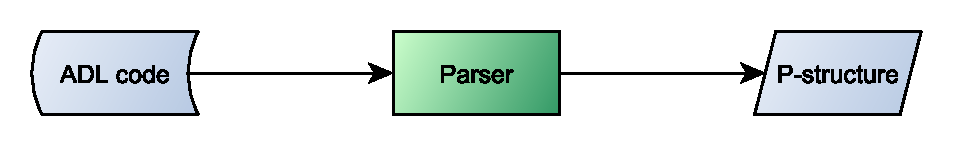
\includegraphics[width=0.586\textwidth]{Figures/DataFlow1}
	\caption{Relevant data flow for the Ampersand parsing component}
	\label{fig:data-flow-1}
\end{figure}

Often, the parsing component is separated into a lexer (that converts text to tokens) and the actual parser (that converts the tokens into the parse tree).
Since this separation is considered beneficial for both maintainability and performance \citeac{parsec}, we assumed from the beginning that the new Ampersand parser would be separated in this way.
This is depicted in \autoref{fig:data-flow-2}.
The previous parser also had a separate lexer, but the name was scanner instead.
%
\begin{figure}[htb!]
	\centering
	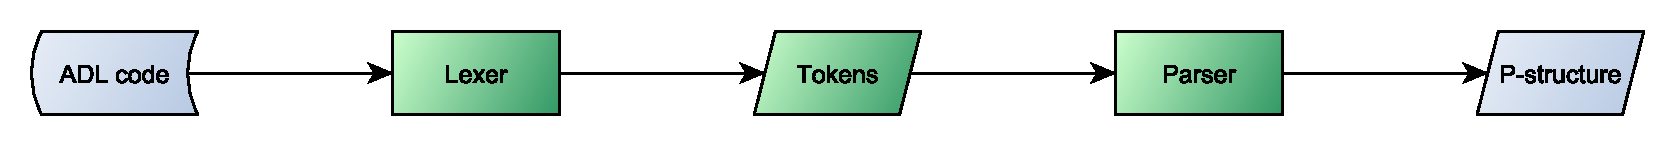
\includegraphics[width=1\textwidth]{Figures/DataFlow2}
	\caption{Data flow for the Ampersand lexing and parsing components}
	\label{fig:data-flow-2}
\end{figure}

In order to take the next steps and understand how the parser can be designed, we first take a look at the grammar in \autoref{subsec:analysis-grammar} and the parse tree in \autoref{subsec:analysis-parse-tree}.
Afterwards, we analyze the lexer with the original token structure, so that we can define a new token structure, in \autoref{subsec:analysis-lexer}.
Finally, we analyze the parser in \autoref{subsec:analysis-parser} and the generated errors in \autoref{subsec:analysis-errors}.

\subsection{Grammar (M)}
\label{subsec:analysis-grammar}
\dict{EBNF}{Extended Backus-Naur Form}%
\dict{Extended Backus-Naur Form}{Notation technique for documenting context-free grammars}%

\subsection{Getting the EBNF in good shape}
The Ampersand syntax is described using the EBNF notation. 
At the beginning of the project, we noticed that the existing EBNF diagram was not in line anymore with the actual syntax of Ampersand.
As the EBNF is a crucial source of information in building the new parser, the first focus was to update the old EBNF to represent the actual Ampersand Syntax.

Through reverse engineering, we checked all Haskell functions on the actual syntax they implement.
In the source of the new parser, all the syntax notations are placed above the actual parser function to support code maintainability.

The derived, and up to date, syntax is visualized using a railroad diagram, an ideal technique to visualize context free grammars.
Several railroad diagram generators are available on the internet, free of charge.
We used the railroad diagram generator created by Gunter Rademacher, available on http://bottlecaps.de/rr/ui.
During the actual generation, the generator failed on the Ampersand Syntax, more precisely on the statement: Exp4 ::= Exp5 (( ';' Exp5 )* | ('!' Exp5)*)
Convinced of the correctness of the EBNF statement, we contacted the owner of the tool, and he discovered a bug in his tool which he corrected promptly.

\subsection{The actual EBNF diagram}

TODO: Show/describe the EBNF (maybe actual EBNF as attachment).
TODO: Note that this EBNF was not available, but we had to derive it from the parser.
TODO: Note that we helped the railroad site to resolve a bug.

One interesting plus is that during the project we found a bug in the Railroad Diagram Generator.
The tool would crash with the \hyperref[fig:ebnf-Trm4]{\texttt{Trm4}} expressions.
This bug was reported to the author Gunther Rademacher, who promptly fixed the issue.

\subsection{Parse tree (R-M)}
\label{subsec:analysis-parse-tree}
The parse tree (also known as P-structure) is a data structure that very much resembles the EBNF description.
The root of the tree is the \texttt{P\_Context} structure, and every leaf of the tree has a field for the location where it was found in the ADL code (the \texttt{Origin} structure).
The tree is consistently defined with the record syntax and is well documented.

However, the constructions are not completely pure, since some transformations are necessary from the ADL to the P-structure.
This forces the parser to do more than only parsing.
Also, the order of the fields can be confusing; sometimes \texttt{Origin} is the first field and sometimes it is not.

During this project, small changes to the parse tree have been done.
These changes are described in \autoref{subsec:design-parse-tree}.

\subsection{Lexer (M)}
\label{subsec:analysis-lexer}
TODO: describe the possible improvements in the old lexer.

\subsubsection{Token structure}
TODO: Describe the old token strucure

\subsubsection{New token structure}
TODO: Develop a better token structure

\subsection{Parser (R-M)}
\label{subsec:analysis-parser}
The previous Ampersand parser was generally well organized, so each ENBF rule could be mapped to a different parser.
However, several flaws were observed as improvement points.
During this project, we focused on the following issues:
\begin{description}
  \item[Lacking documentation]
    There was no documentation on the recognized grammar.
    The last EBNF available was not updated in a long while.
  
  \item[Ad-hoc transformations]
    The parser was built with the applicative interface of the uulib.
    The applicative operators were thus used in sequence to recognize each of the accepted grammar productions.
    However, the parser was often forced to change the order and format of the parsed structures, because the parse tree did not match the grammar productions (i.e. many rebuild functions).
    
  \item[Long file]
    Since all the grammar constructions -- plus help functions -- were in a single file, the parser was hardly readable.
    It summed a total of 823 lines of code only in the \texttt{Parser} module.
  
  \item[Pretty printing]
    It used to be impossible to print the parse tree back to ADL-code.
    That made it harder to develop and test the parser properly.
  
  \item[Test suite]
    There were no automated tests for the parser.
    Because of this, any code change would be hard to test and could potentially influence other Ampersand modules.
  
  \item[Duplicated code]
    A large part of the code was duplicated and not used (mainly in the \texttt{Parsing} module).
  
  \item[Error messages]
    As mentioned, the main reason for this project was the bad quality of the error messages generated.
    \autoref{subsec:analysis-errors} expands on this point.
\end{description}
%
Although it may be hard to resolve all the mentioned issues, we believe our efforts have played off well.
In \autoref{subsec:design-parser} we describe how the new parser was designed.

\subsection{Errors (M)}
\label{subsec:analysis-errors}
TODO: show how the parser did not provide good errors, and how we could improve them.

% !TEX root = ../Documentation.tex

\section{Design}
\label{sec:design}

\subsection{System overview (D)}
  The parser module overview is given in \autoref{fig:ParserModules}.
  Each of the modules are described in the following subsection.
  %
  \begin{figure}[ht]%
    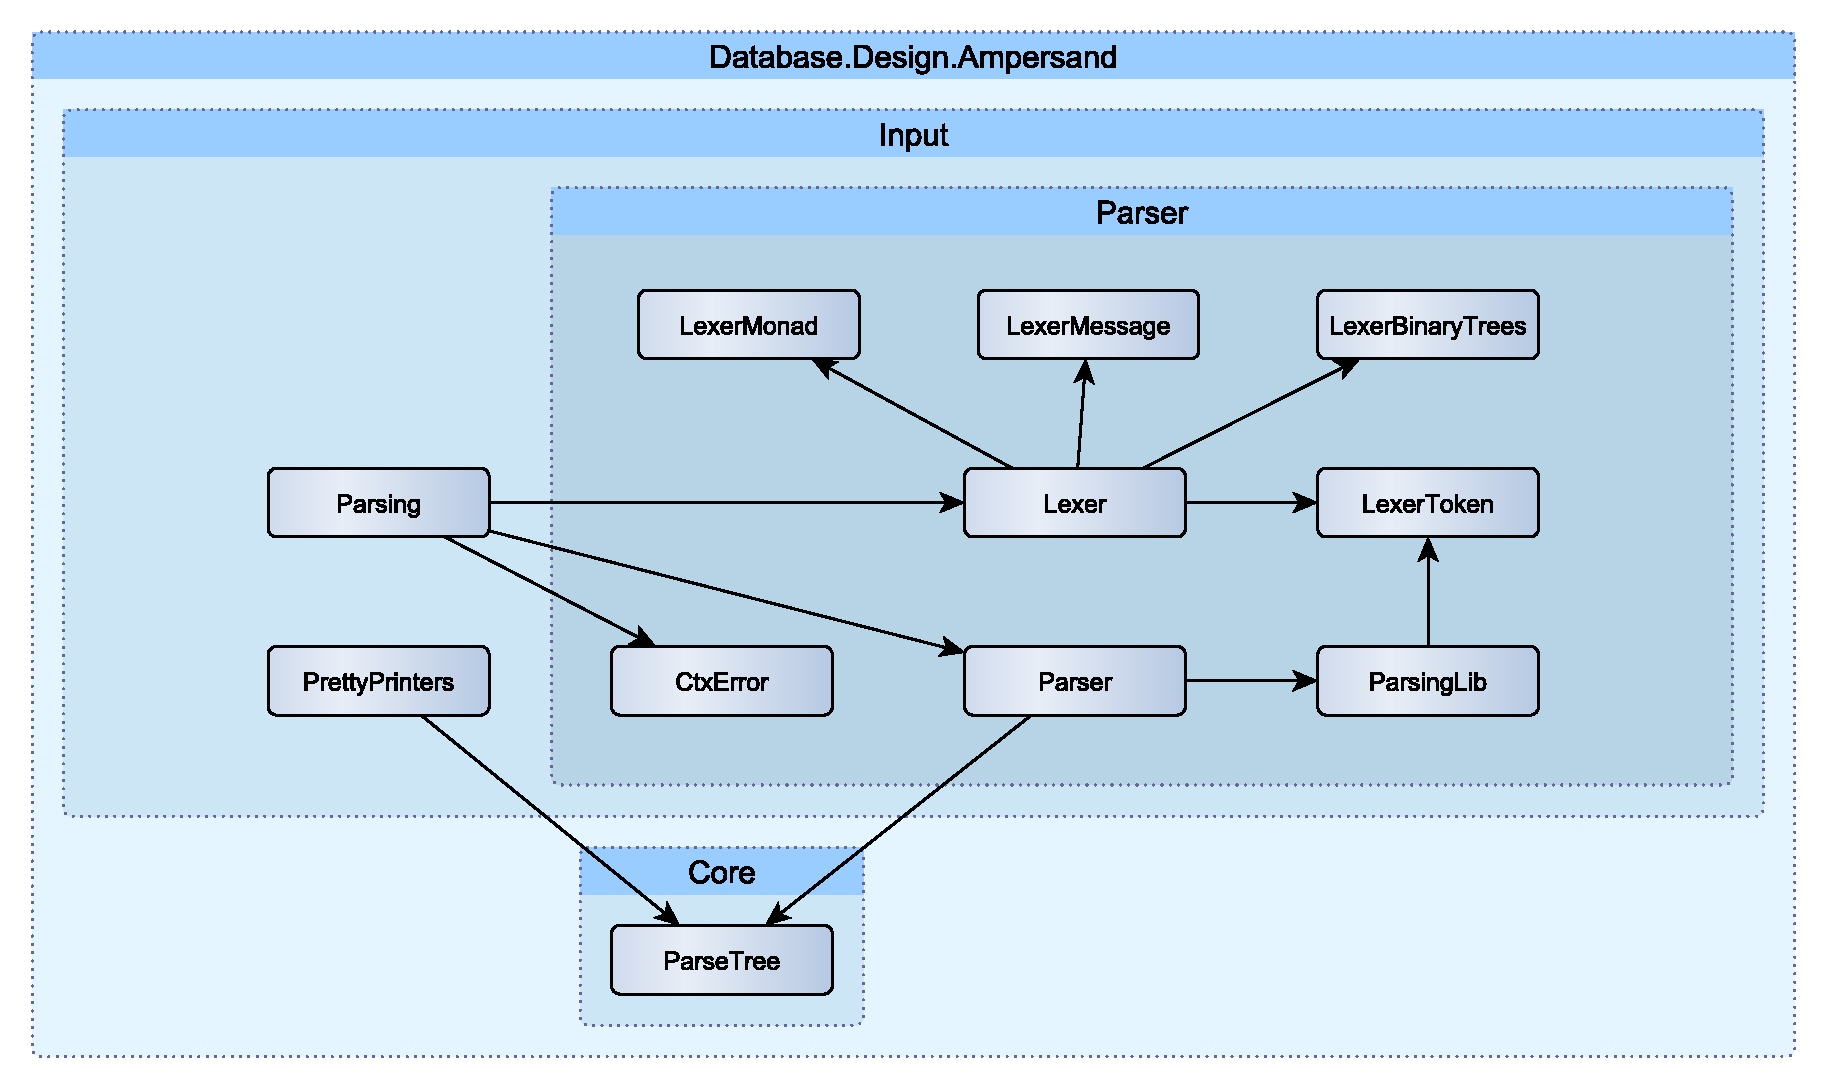
\includegraphics[width=\columnwidth]{Figures/ParserModules}
    \caption{The parser modules and their relationships}
    \label{fig:ParserModules}
  \end{figure}%
  TODO: Add the exported functions to each module.

  \subsubsection{Modules}
  \label{subsec:parser-modules}
  In this section a short description of each module is given:
  %
  \begin{description}
    \item[Parsing] module that implements the interface of the parser with the rest of the system.
      It is responsible for reading the input files, calling the lexer and the parser and returning a parse tree as result (or a parse error).

    \item[Parser] module responsible for executing the parsing itself.
      It accepts the tokens that are allowed in each grammar production and generates the corresponding parse tree.
      The parser is described in \autoref{subsec:design-parser}.
      
    \item[ParsingLib] library that contains several useful functions to assist the parser, e.g. token recognition.
      These functions are not depending on the specific grammar rules.
      
    \item[ParseTree] external module containing the parse tree data structures.
      Only details of this module have been changed during this project (e.g. field ordering).
    
    \item[PrettyPrinters] contains the \texttt{Pretty} class and the functions responsible for printing the parse tree to ADL scripts in a `pretty' way.
    
    \item[CtxError] contains the data structures responsible for the parse errors and their location.
      This module has not been refactored as a part of this project.
    
    \item[Lexer] module responsible for recognizing the input characters and converting them to tokens.
      The lexer, together with its sub-modules, is described in \autoref{subsec:lexer}.
  \end{description}

\subsection{Lexer (M)}
\label{subsec:lexer}
The lexer module is responsible to split up the input stream into tokens.
Tokens are meaningful pieces of the input strings that needs to be kept together together.

\subsubsection{The rationale behind the new lexer}
In the design of the new Ampersand parser, the question arose whether to keep the current scanner or to implement a new one.
After the analysis of the error improvement areas, the main improvements were identified within the actual parser.
The error feedback quality produced by the scanner module was higher and therefore, there was no stringent need to re-implement the scanner.
On the other hand, given the aspect that Parsec was defined as the new Parser library, keeping the current scanner would have resulted in the utilization of 2 different libraries providing more of less the same functionality.
To avoid a decrease in maintainability, the decision is made to implement the parser and scanner based on the same library.
During the implementation of the lexer module, replacing the old scanner, additional attention was given to further improve the quality of the error messages
The scanner module is renamed to the lexer module to stress the aspect that the principle of lexemes is used in the new scanner.

The lexer is build based on the existing Helium lexer modules. 
One of the main goals of this project create a compiler and a dialect of Haskell in which clear error messages were produced. TODO: reference
The Lexer module in Helium contains interesting principles such as position monitoring, warnings and easy maintainable error messages.


\subsubsection{Lexer structure}


The lexer is the main module, in which the actual lexing is done, and to do so, it it using the following sub-modules:

 \begin{description}
 
    \item[LexerMonad] contains a monad definition that supports lexing with context.
      It tracks for example the location in the input and the warnings that may be generated.
	  This module is re-used without any modification out of the  Helium parser.
      The following functions or types are used in the Ampersand lexer:
	  \begin{itemize}
		\item [LexerMonad] is the main monadic type used in the lexer returning an error or a list of tokens together with a list of warnings
		\item [addPos] is used to trace the position of the token
		\item [lexerError] to generate lexer error
		\item [lexerWarning] to generate lexer warnings
		\item [runLexerMonad] main function to handle the LexerMonad results 
	  \end{itemize}
	  
    \item[LexerMessage] contains functions to handle errors and warnings from the lexer.
	  Based on the warning/error type and the needed language, LexerMessage will fetch the correct description of an error or a warning out of the LexerTexts module
	  The show functions for the error and warning are maintained in this module.
	  
    \item[LexerTexts] will fetch the correct description of an error or a warning out of the LexerTexts module.
	  This centralisation provides an easy entry point for the maintenance of the actual messages as the actual messages are no longer dispersed over the module functions.
	  
    \item[LexerBinaryTrees] module responsible for searching binary trees in an efficient way, to support the token recognition.
            This is the existing UU_BinaryTrees module which is renamed to match the used naming structure of the new lexer modules.

    \item[LexerToken] contains the data structure, and corresponding show function, that represents the input tokens for the lexer.
	
  \end{description}

Each token contains a part of the input string together with an identifier, defining the token content, and the position of the token in the input file.
The token structure is defined as follows:

data Token = Tok \{	  tokLex :: Lexeme
                		, tokPos :: FilePos \}

The lexeme is the combination of the token type and the actual token content, sliced from the input string.
FilePos is used to keep track of the original position of the lexeme in the input string.

During the lexer processing, the input file is processed sequentially.
All kind of differentiating formats are checked in a specific order, and each time a match is found, the lexeme is extracted from the input file and the token is created.
In the token creation, function ReturnToken, the position and lexeme is grouped into the actual token and the next nested lexer iteration is launched.


\subsection{Parser (R-M)}
\label{subsec:design-parser}
The mainstream design of the new parser has not changed much.
Basically, each EBNF rule receives its own parser function.
Thanks to the combinator operators, each parsing function also looks very similar to its corresponding EBNF.

The applicative interface is consistently used.
By changing details of the implementation, e.g. the order of the fields in the parse tree, we have made many of the `rebuild' functions unnecessary.
For some parsers the amount of changes necessary in order to remove supporting functions was too large or even impossible with the current parse tree.

Note that in parts of the parser, the function syntax has substituted the record syntax for creating data objects.
This was done only when the code readability could be improved by doing so.

\subsubsection{Parsec}
\label{subsec:design-parsing-lib}
As mentioned earlier, and described in research context document \citenac{parsing}, the new Ampersand parser has been rebuilt with another parsing library, namely Parsec.
However, for the Ampersand developers, the source code of the parser will still look very familiar, thanks to the applicative interface.
For developers, the main differences between Parsec and the uulib are:
\begin{itemize}
  \item Parsec does not backtrack by default.
    In order to enable backtracking, the \texttt{try} function must be used.
    This is described in \autoref{subsec:backtracking}.
  \item Parsec does not try to solve parsing errors.
    The parser stops immediately after the first issue.
    See also the error analysis in \autoref{subsec:design-errors}.
  \item Error messages are customizable by using the \texttt{<?>} operator.
    This is also suggested in \autoref{subsec:design-next-steps}.
  \item Some combinators have a different name, e.g. one must use \texttt{option} instead of \texttt{opt}.
    Assuming the documentation found on Hackage is clear and sufficient, interface differences are not documented here.
\end{itemize}

\subsubsection{Backtracking}
\label{subsec:backtracking}
In order to explain the differences on backtracking behavior between the uulib and Parsec, we quote here Doaitse Swierstra, the author of the uulib \citenac{swierstra-parsec}:
\begin{quote}
\textsl{To understand the subtleties it is important to understand the differences between the try construct in Haskell and the non-greedy parsing strategy used in uu-parsinglib. Effectively the latter is a try which just looks ahead one symbol. In that respect it is less powerful than the try construct from Parsec, in which you specify that a specific construct has to be present completely. And then there is the underlying different overall strategy. Parsec uses a back-tracking strategy with explicit tries to commit, whereas uu-parsinglib uses a breadth-first strategy with an occasional single symbol look-ahead.}
\end{quote}
%
We can therefore conclude that the try-statements in Parsec are undesirable.
However, they are necessary when the grammar is ambiguous.
In this section we explain why each of the remaining try statements are necessary, and how these issues can be resolved:
\begin{description}
  \item[Classify]
    This ambiguity in the grammar arises from the \texttt{Classify} and \texttt{GenDef} productions:
    \begin{quote}
        \texttt{Classify ::= `CLASSIFY' ConceptRef `IS' Cterm}\\
        \texttt{GenDef ::= (`CLASSIFY' | `SPEC') ConceptRef `ISA' ConceptRef}
    \end{quote}
    When the parser encounters \texttt{`CLASSIFY'}, it cannot define whether it found a \texttt{Classify} or a \texttt{GenDef} production.
    Therefore, the parser must consume the keyword and a \texttt{ConceptRef} before consuming either \texttt{`IS'} or \texttt{`ISA'} and determining which production is applicable.
    
    In order to solve this issue, one must choose a different keyword or symbol for each of the productions.
    Another option would be to merge the two statements in the same parser.
    We did not merge the productions because that would make the parser less maintainable.
  
  \item[Role]
    This ambiguity in the grammar arises from the \texttt{RoleRelation} and \texttt{RoleRule} productions:
    \begin{quote}
        \texttt{RoleRelation ::= `ROLE' RoleList `EDITS' NamedRelList}\\
        \texttt{RoleRule ::= `ROLE' RoleList `MAINTAINS' ADLidList}
    \end{quote}
    When the parser encounters \texttt{`ROLE'}, it cannot define whether it is a \texttt{RoleRelation} or a \texttt{RoleRule} production.
    Therefore, the parser must consume the keyword and a \texttt{RoleList} (which may be long) before consuming either \texttt{`MAINTAINS'} or \texttt{`EDITS'} and determining which production is applicable.
    
    In order to solve this issue, one must choose a different keyword for each of the productions, merge the two options to have the same representation in the parse tree, or refactor the parser so that the two options are parsed together.
    We did not merge the productions because that would make the parser less maintainable.
  
  \item[View]
    This ambiguity in the grammar arises from the \texttt{FancyViewDef} and \texttt{ViewDefLegacy} productions:
    \begin{quote}
        \texttt{FancyViewDef ::= `VIEW' Label ConceptOneRefPos `DEFAULT'? `\{' ViewObjList `\}' HtmlView? `ENDVIEW'}\\
        \texttt{ViewDefLegacy ::= (`VIEW' | `KEY') LabelProps ConceptOneRefPos `(' ViewSegmentList `)' }
    \end{quote}
    When the parser encounters \texttt{`VIEW'}, it cannot define whether it found a \texttt{FancyViewDef} or a \texttt{ViewDefLegacy} production.
    In this case, defining which construction is applicable is even more complicated.
    This decision must, in the worst case, be delayed until the parser encounters a \texttt{`\{'} or \texttt{'('}.
    That's because the productions \texttt{Label} and \texttt{LabelProps} are not disjoint, and \texttt{`DEFAULT'} is optional.
    
    In order to solve this issue, we advise to merge or drop the legacy statement.
    
  \item[Multiplicity]
    This ambiguity in the grammar arises from the \texttt{Mult} production:
    \begin{quote}
        \texttt{Mult ::= (`0' | `1') `..' (`1' | `*') | `*' | `1'}
    \end{quote}
    When the parser encounters \texttt{`1'}, it cannot define whether it found the first or the last production.
    The parser must therefore read the next token before choosing the right option.
    
    In order to solve this issue, we advise to refactor the grammar (and the parser) to have the following production:
    \begin{quote}
        \texttt{Mult ::= `0' `..' (`1' | `*') | `1'(`..' (`1' | `*'))? | `*'}
    \end{quote}
    %
    We did not refactor the code in this matter because the \texttt{pMult} parser does more than only parsing: it also changes the representation of the found constructions before creating the parse tree.
  
  \item[Labels and Terms]
    In the productions \texttt{IndAtt}, \texttt{ViewAtt} and \texttt{RuleDef}, we see very similar ambiguities:
    \begin{quote}
        \texttt{IndAtt ::= LabelProps? Term}\\
        \texttt{ViewAtt ::= LabelProps? Term}\\
        \texttt{RuleDef ::= `RULE' Label? Rule Meaning* Message* Violation?}
    \end{quote}
    Wherein:
    \begin{quote}
        \texttt{Label ::= ADLid ':'}\\
        \texttt{LabelProps ::= ADLid (`{' ADLidListList `}')? `:'}\\
        \texttt{Rule ::= Term ('=' Term | '|-' Term)?}
    \end{quote}
    And one of the possible productions of \texttt{Term} is:
    \begin{quote}
        \texttt{Term ::= Trm2 ::= Trm3 ::= Trm4 ::= Trm5 ::= Trm6 ::= RelationRef ::= NamedRel ::= Varid Sign?}
    \end{quote}
    While:
    \begin{quote}
        \texttt{ADLid ::= Varid | Conid | String}
    \end{quote}
    
    What happens here is that when the parser encounters a \texttt{Varid}, it cannot define whether it is part of the (optional) \texttt{Label} production or if no \texttt{Label} was given and the \texttt{Varid} is part of a \texttt{Term}/\texttt{NamedRel} production.
    
    Due to the quite complex grammar for the \texttt{Term} production, this issue may severely impact the parser's performance.
    This is probably the most harmful of the ambiguities mentioned.
    However, it can only be solved by adding a symbol before the \texttt{Term} production (e.g. making the `:' non-optional).
    
    \textbf{TODO: IndAtt and ViewAtt are the same parser.}
\end{description}
%
Please note that in order to have proper backtracking with correct error messages, Parsec may require two try-statements \citenac{try-harmful}.

\subsection{Parse tree (R-M)}
\label{subsec:design-parse-tree}
Improvements in the Ampersand parse tree are out of the scope of this project, because of the potential consequences to the rest of the Ampersand system.
However, during the development of the new parser a few constructions have been changed in order to make the parser more readable and maintainable.
The changes have been mostly in the order of the constructor parameters, and this was done consequently though all Ampersand modules.
The updated parse tree is depicted in the appendices (\autoref{fig:parse-tree}).

\subsection{Errors (M)}
\label{subsec:design-errors}
TODO: show what we've done to improve the errors.

\subsection{Next steps (M)}
\label{subsec:design-next-steps}
TODO: give tips on how to further improve the parser. e.g.:
  - cleanup CtxError, add warnings, use <?> for the errors.
  - reorganize parse tree, e.g. using always Origin as first parameter.
% !TEX root = ../Documentation.tex

\section{Test Report}
\label{sec:tests}

\subsection{Test suite}
  Together with the new parser, a test suite has been developed.
  This test suite has been used to verify the performance and correctness of the new parser.
  The source code can be found in the folder \texttt{src/Database/Design/Ampersand/Test} within the Ampersand repository.

  The test suite runs in three steps, which are depicted in \autoref{fig:TestModules}.
  Each of the modules are described in the following subsection.
  %
  \begin{figure}[ht]%
    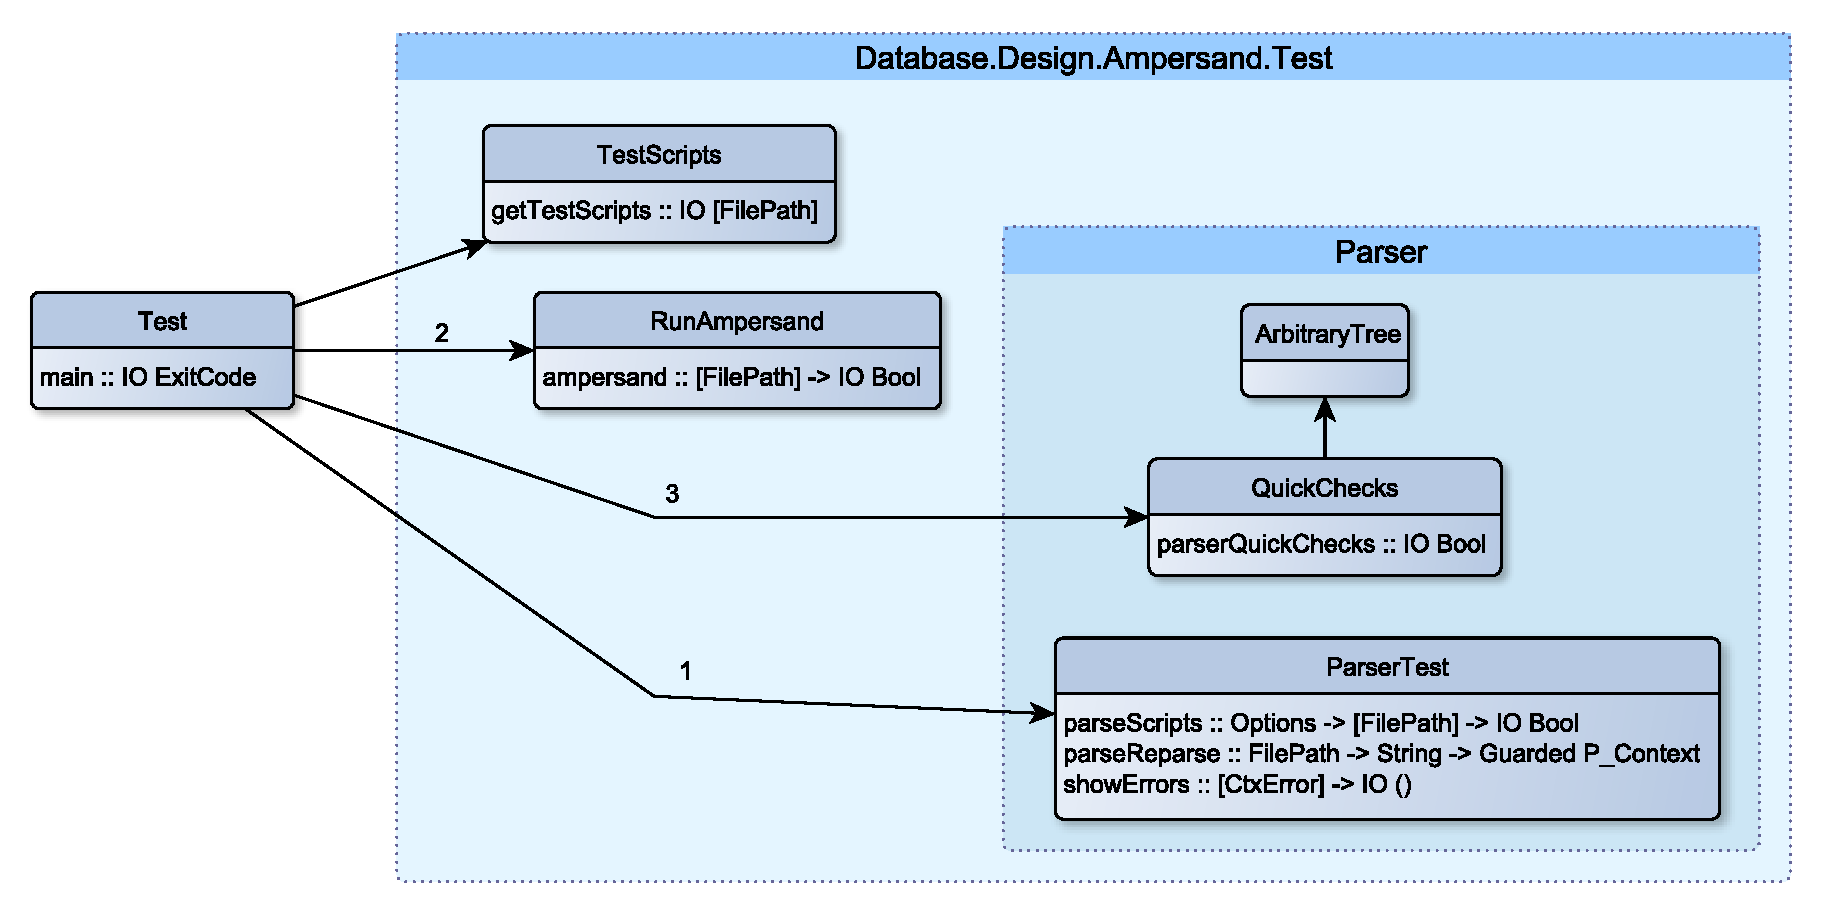
\includegraphics[width=\columnwidth]{Figures/TestModules}
    \caption{Test suite modules with their exported functions}
    \label{fig:TestModules}
  \end{figure}%

  \subsubsection{Modules}
  \label{subsec:test-modules}
  In this section a short description of each module is given:%
  %
  \begin{description}
    \item[Test] contains the \texttt{main} method that can be executed to run the test suite.
      The \texttt{main} function calls each of the other modules in sequence, stopping if any of them returns \texttt{False}.
      When all tests have been successful, the return code is \texttt{ExitSuccess}.
      Otherwise, the return code is naturally \texttt{ExitFailure}.
    
    \item[TestScripts] retrieves a list of scripts that can be used for the different tests.
      It searches for tests within the folder \texttt{ArchitectureAndDesign}, and contains a list of scripts from the \texttt{ampersand-models} repository, that can be changed at a later moment if wished.
      Note that all the ADL-scripts listed in this section must be correct for the parser and the type checker.
    
    \item[ParserTest] exports three functions that are the core of testing the parser:
      \begin{itemize}
        \item \texttt{parseScripts} receives a list of files to parse, and checks that every file can be parsed successfully.
        \item \texttt{parseReparse} tries to parse a file, and if sucessfull, pretty-prints the result and parses it again.
        \item \texttt{showErrors} prints the given parse errors to the output.
      \end{itemize}
    
    \item[RunAmpersand] receives a list of files, and checks that every file can be executed successfully by Ampersand.
      This tests thus not only the parser, but also the interface between the parser and the type checker, as the rest of the Ampersand chain.
    
    \item[QuickChecks] generates random parse tree structures and generates the corresponding ADL-script by pretty printing the parse tree.
      This ADL-script is then fed back to the parser through the \texttt{parseReparse} function, to verify that the parser can accept any random input.
      More information on the quick checks is given in subsection~\ref{subsec:quick-check}.
    
    \item[ArbitraryTree] is a support module that gives \texttt{Arbitrary} instances to all parse-tree structures.
      This is used by QuickCheck as described in subsection~\ref{subsec:quick-check}.
    
    \item[ArbitraryPandoc] contains \texttt{Arbitrary} instances to the Pandoc data types.
      This file has not been developed in this project, but copied from the \texttt{jgm/pandoc} project with the GPL license.
  \end{description}

  \subsubsection{QuickCheck and pretty printing}
  \label{subsec:quick-check}
  The most innovative part of the test suite is the use of random structures to test the parser.
  In this section we describe how this generation is implemented.
  
  The main role in the generation of random structures is played by the support library QuickCheck, which has been added to the Ampersand project.
  QuickCheck is able to generate any data structure randomly.
  However, since the parse tree is a custom structure that must obey specific rules, QuickCheck requires the specification of these rules by instances of the \texttt{Arbitrary} class.
  
  Every data structure in the parse tree has received an \texttt{Arbitrary} instance used for test purposes.
  The instances can be found in the module \texttt{Database.Design.Ampersand.Test.Parser\-.ArbitraryTree}, as described in subsection~\ref{subsec:test-modules}.
  
  After generating the random parse trees, the test suite needs to convert them to ADL-scripts.
  The conversion of parse tree to source code is also known as pretty printing.
  As the pretty printing is seen as part of the parse tree, it is not included in the Test modules, but is part of the input subsystem.
  The pretty printing instances are found in the module \texttt{Database.Design.Ampersand.ADL1.PrettyPrinters}.
  This module makes use of the library \texttt{Text.PrettyPrint.Leijen}, that outlines the output so it is indeed `pretty'.
  
  Now that the ADL source is available, the parser is executed.
  The result of the parser is checked to be equal to the generated tree by the property \texttt{prop\_pretty}.
  The property is currently tested for 64 generated parse trees in the test suite.
  If the test fails for any generated structure, the test suite fails with an appropriate error.
  
  \subsubsection{Running the tests}
  During the parser development, the \texttt{main} function of the parser tests has been executed manually, through a batch file.
  This is mainly done because the project team did not have access to the Sentinel server, and no documentation was available on how to run Sentinel locally in a Windows machine.
  However, now that the parser is being delivered, it should be integrated with the other existing Ampersand/Sentinel tests.
  We leave the option open for the Ampersand development team to either add the Sentinel jobs to this test suite, or to add the parser test suite to the Sentinel jobs.
  
\subsection{Errors}
  Since evaluating the quality of error messages is manual work, the errors have not been included in the test suite.
  TODO: Give Maarten's findings on how the errors have improved. Maybe the tables should be an attachment, but the summary should be here.

\subsection{Next steps}
  In this section we name a couple changes that can be done in the test suite in the future:
  \begin{description}
    \item[Sentinel] During the development of the new parser, we worked in a separate fork.
      Our changes were not being tested in the Ampersand test server (Sentinel).
      Since we did not have access to this server, we developed a separate test suite.
      It may be pertinent to integrate the Sentinel jobs into the test suite or to integrate the test suite into the Sentinel jobs.
    
    \item[Output] Currently, the test suite outputs errors by using the \texttt{Debug.Trace} module.
      From a purely functional perspective, using this module may be undesirable.
      Therefore, the Ampersand team may consider changing the test outputs to use IO with monads in a more functional way.
  \end{description}


\newpage
% !TEX root = ../Parsing.tex

\section{Conclusion}
\label{sec:conclusion}
In \autoref{sec:libraries}, the advice was given to use a combinator library for the new parser of Ampersand.
The main reason to avoid the parser generators is that it is hard to generate useful feedback.
Then, in \autoref{sec:errors}, it was made even more clear that besides generating good messages, those messages should also be customizable.

Therefore, the advice of this research is to use the combinator library that offers the highest level of customization in error messages, Parsec.
Although the uu-parsinglib seems to also be a very good choice, the experiences from the Helium compiler \citeac{helium-parser} should be also considered.
Besides, the Parsec library offers better support.

A list of important consideration points has also been collected through the literature and can be found in \autoref{sec:errors}, more specifically \ref{subsec:errors-ampersand}.
\newpage

\part*{Appendices}
\addcontentsline{toc}{part}{Appendices}
\appendix
% !TEX root = ../Parsing.tex

\small
\printglossary[style=mcolindex,title=Glossary]
\label{sec:glossary}

\newpage
\begin{landscape}

  \section*{Parse Tree}
  \label{app:parse-tree}
  \addcontentsline{toc}{section}{Parse Tree}
  \begin{figure}[htb!]
    \centering
    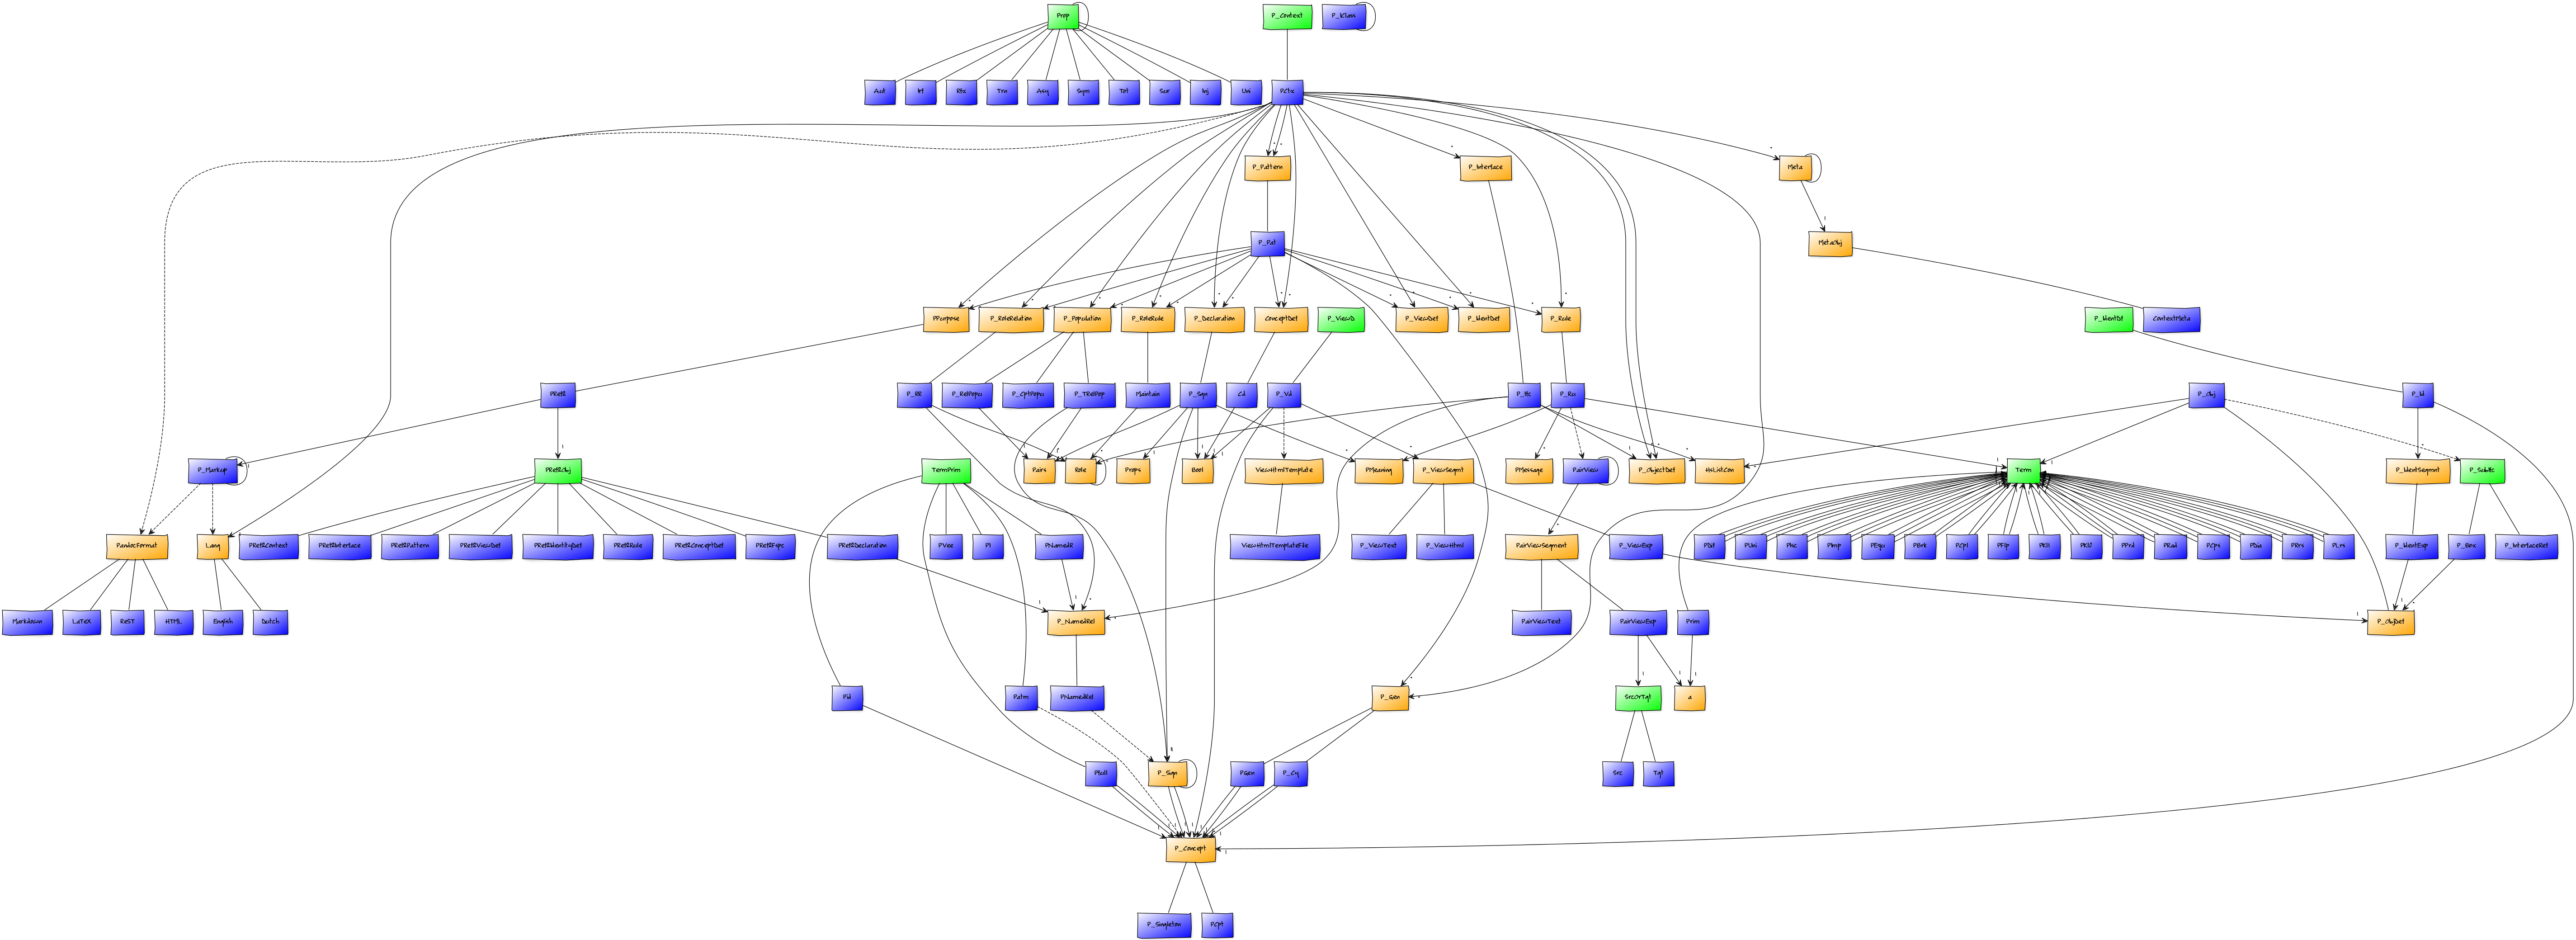
\includegraphics[width=25.4cm]{Figures/GenParseTree}
    \caption[Diagram of the Ampersand parse tree]{
      Diagram of the Ampersand parse tree. \small
      %Data definitions are depicted in green, constructors are depicted in blue and 
      Connections without an arrow represent the data contructors.
      Connections with an arrow also show the multiplicity in the relationship (i.e. 1 or *) or are stripped to represent an optional relationship.
      }
    \label{fig:parse-tree}
  \end{figure}

\end{landscape}
\newpage
% !TEX root = ../Parsing.tex
\addcontentsline{toc}{section}{References}
\label{sec:bibliography}

\begin{thebibliography}{99}

\bibitem{plan}
	Planning for the project `Useful feedback in the Ampersand parser'\\
	Maarten Baertsoen and Daniel S. C. Schiavini\\
	Version 2.0 -- November 29, 2014\\
	\url{http://git.io/NeHuLg}

\bibitem{heeren-error}
	Top Quality Type Error Messages\\
	Bastiaan Heeren\\
	ISBN 90-393-4005-6, September 20, 2005\\
	\url{http://www.open.ou.nl/bhr/phdthesis}

\bibitem{monadic-parsing}
	Functional pearls -- Monadic Parsing in Haskell\\
	Graham Hutton (University of Nottingham) and Erik Meijer (University of Utrecht)\\
	\url{http://www.cs.nott.ac.uk/~gmh/monparsing.pdf}

\bibitem{convert-ebnf}
	 From EBNF to BNF \\
	 Christoph Zenger\\
	 June 4, 2000\\
	 \url{http://lampwww.epfl.ch/teaching/archive/compilation-ssc/2000/part4/parsing/node3.html}

\bibitem{bnf-ebnf}
	BNF and EBNF: What are they and how do they work?\\
	Lars Marius Garshol\\
	August 22, 2008\\
	\url{http://www.garshol.priv.no/download/text/bnf.html}

\bibitem{parser-examples}
	Haskell Parser Examples\\
	Geoff Hulette\\
	August 22, 2014\\
	\url{https://github.com/ghulette/haskell-parser-examples}

\bibitem{hugs-parser}
	Source code of the Hugs parser\\
	March 25, 2007\\
	\url{https://github.com/fuzxxl/Hugs/blob/master/src/parser.y}

\bibitem{ghc-parser}
	GHC: The Parser\\
	December 1, 2014\\
	\url{https://ghc.haskell.org/trac/ghc/wiki/Commentary/Compiler/Parser}
	%\url{https://ghc.haskell.org/trac/ghc/browser/ghc/compiler/parser/Parser.y}
	%https://www.haskell.org/pipermail/haskell-cafe/2013-August/109557.html

\bibitem{helium-parser}
	Helium, for Learning Haskell\\
	Bastiaan Heeren, Daan Leijen, Arjan van IJzendoorn\\
	Utrecht University\\
	\url{http://www.open.ou.nl/bhr/heeren-helium.pdf}
	
\bibitem{gcc-c-parser}
	GCC 4.1 Release Series Changes, New Features, and Fixes\\
	\url{https://gcc.gnu.org/gcc-3.4/changes.html}

\bibitem{gcc-cpp-parser}
	GCC 3.4 Release Series Changes, New Features, and Fixes\\
	\url{https://gcc.gnu.org/gcc-4.1/changes.html}
	
\end{thebibliography}

\end{document}
\clearpage
% !TEX root = ../Planning.tex
\section{Tools, methodologies and accelerators}
\label{sec:tools-methodologies}

\subsection{Collaboration}
\dict{Dropbox}{File hosting service that offers cloud storage, file synchronization, personal cloud, and client software}%
\dict{Git}{A distributed revision control and source code management}%
\dict{GitHub}{Git repository web-based hosting service which offers all of the distributed revision control and source code management (SCM) functionality of Git}%
\dict{Microsoft Office}{Office suite of desktop applications developed by Microsoft}%
For the collaboration between the project members, the following tools will be used:
\begin{description}
	\item[Dropbox] For sharing time tracking and other reference documents;
	\item[GitHub] For sharing git repositories of code, besides managing issues and documentation;
	\item[SourceForge] For managing existing issues with the customer and other developers;
	\item[Microsoft Office] For writing internal documents, e.g. time tracking;
\end{description}

\subsection{Documentation}
\dict{Haddock}{A software documentation generator for the Haskell programming language}%
\dict{TeXworks}{Graphical user interface for editing and compiling \LaTeX{} documents}%
\dict{LaTeX}{Document preparation system and document markup language for the TeX typeset}%
\dict{RDG}{Railroad Diagram Generator}%
\dict{Railroad Diagram Generator}{Tool for generating syntax diagrams based on EBNF notation}%
\dict{EBNF}{Extended Backus-Naur Form}%
\dict{Extended Backus-Naur Form}{Notation technique for documenting context-free grammars}%
For writing the documentation, the following tools will be used:
\begin{description}
	\item[Haddock] For annotating documentation on the code;
	\item[TeXworks] For writing, editing and compiling \LaTeX{} documents;
	\item[Ampersand Wiki] For keeping notes and information useful for users and other developers;
	\item[Railroad Diagram Generator] For generating syntax diagrams based on EBNF notation.
\end{description}

\subsection{Design}
\dict{yEd}{Software for editing graphs}%
For designing the software and its architecture, the following tools will be used:
\begin{description}
	\item[yEd] For creating diagrams and graphs;
\end{description}

\subsection{Development}
\dict{IDE}{Integrated Development Environment}%
\dict{GHC}{Glasgow Haskell Compilation system}%
\dict{Cabal}{Library for managing Haskell builds and packages}%
For software development, the following tools will be used:
\begin{description}
	\item[IDE] No standard integrated development environment will be chosen: the project members are free to use any IDE, e.g. Eclipse, Leksah, Notepad++;
	\item[GHC] The compiler GHC (Glasgow Haskell Compilation System), version 7.8.3, will be used;
	\item[Cabal] For managing Haskell packages and compilation, cabal-install version 1.18.0.5 and Cabal library version 1.18.1.3.
\end{description}

\subsection{Testing}
\dict{Hpc}{Library for checking, recording and displaying code coverage}%
\dict{Sentinel}{Test server for the Ampersand project}%
\dict{QuickCheck}{Library for testing Haskell code}%
\dict{HLint}{Library that reads Haskell programs and suggests changes that hopefully make them easier to read}%
Finally, the following tools are selected to be used, where appropriate, for testing the software:
\begin{description}
	\item[Hpc] might be used for checking, recording and displaying the code coverage of tests;
	\item[Sentinel server] can be used for the integration tests;
	\item[QuickCheck] for automating tests on the code and property based testing (e.g. pretty-print and reparsing, random code generation);
	\item[Neil Mitchell's HLint] for checks on the code readability and maintainability;
\end{description}

\clearpage
\appendix
% !TEX root = ../Parsing.tex

\small
\printglossary[style=mcolindex,title=Glossary]
\label{sec:glossary}

\clearpage
% !TEX root = ../Parsing.tex
\addcontentsline{toc}{section}{References}
\label{sec:bibliography}

\begin{thebibliography}{99}

\bibitem{plan}
	Planning for the project `Useful feedback in the Ampersand parser'\\
	Maarten Baertsoen and Daniel S. C. Schiavini\\
	Version 2.0 -- November 29, 2014\\
	\url{http://git.io/NeHuLg}

\bibitem{heeren-error}
	Top Quality Type Error Messages\\
	Bastiaan Heeren\\
	ISBN 90-393-4005-6, September 20, 2005\\
	\url{http://www.open.ou.nl/bhr/phdthesis}

\bibitem{monadic-parsing}
	Functional pearls -- Monadic Parsing in Haskell\\
	Graham Hutton (University of Nottingham) and Erik Meijer (University of Utrecht)\\
	\url{http://www.cs.nott.ac.uk/~gmh/monparsing.pdf}

\bibitem{convert-ebnf}
	 From EBNF to BNF \\
	 Christoph Zenger\\
	 June 4, 2000\\
	 \url{http://lampwww.epfl.ch/teaching/archive/compilation-ssc/2000/part4/parsing/node3.html}

\bibitem{bnf-ebnf}
	BNF and EBNF: What are they and how do they work?\\
	Lars Marius Garshol\\
	August 22, 2008\\
	\url{http://www.garshol.priv.no/download/text/bnf.html}

\bibitem{parser-examples}
	Haskell Parser Examples\\
	Geoff Hulette\\
	August 22, 2014\\
	\url{https://github.com/ghulette/haskell-parser-examples}

\bibitem{hugs-parser}
	Source code of the Hugs parser\\
	March 25, 2007\\
	\url{https://github.com/fuzxxl/Hugs/blob/master/src/parser.y}

\bibitem{ghc-parser}
	GHC: The Parser\\
	December 1, 2014\\
	\url{https://ghc.haskell.org/trac/ghc/wiki/Commentary/Compiler/Parser}
	%\url{https://ghc.haskell.org/trac/ghc/browser/ghc/compiler/parser/Parser.y}
	%https://www.haskell.org/pipermail/haskell-cafe/2013-August/109557.html

\bibitem{helium-parser}
	Helium, for Learning Haskell\\
	Bastiaan Heeren, Daan Leijen, Arjan van IJzendoorn\\
	Utrecht University\\
	\url{http://www.open.ou.nl/bhr/heeren-helium.pdf}
	
\bibitem{gcc-c-parser}
	GCC 4.1 Release Series Changes, New Features, and Fixes\\
	\url{https://gcc.gnu.org/gcc-3.4/changes.html}

\bibitem{gcc-cpp-parser}
	GCC 3.4 Release Series Changes, New Features, and Fixes\\
	\url{https://gcc.gnu.org/gcc-4.1/changes.html}
	
\end{thebibliography}

\end{document}